\documentclass[12pt]{report}

% Packages
% ========
\usepackage[letterpaper, portrait, margin=1in]{geometry}
\usepackage{graphicx}			% So we can load figures with "." in their filename
\usepackage{float}				% So we can use "[H]"
\usepackage[dvipsnames]{xcolor}	% For custom colors
\usepackage{xparse}				% For \DeclareDocumentCommand
\usepackage{caption}			% For \captionof command
\usepackage{mathtools}			% For \DeclarePairedDelimeter
\usepackage{ifthen}				% For \ifthenelse{}{}{}
\usepackage{soul}				% For underlining with \ul
\setuldepth{x}					%	""
\usepackage{multicol}			% For multiple columns via \begin{multicols}{2}
\usepackage[most]{tcolorbox}	% For the tl; dr environment
\usepackage{array}				% For extended column definitions
\usepackage{tabularray}			% For \begin{longtblr} tables that span multiple columns and pages
\usepackage{amssymb}			% For $\checkmark$
\usepackage{etoc}				% For \localtableofcontents


% Inserting code into LaTeX: \begin{lstlisting} ...
\usepackage{listings}
\definecolor{dkgreen}{rgb}{0,0.6,0}
\definecolor{gray}{rgb}{0.5,0.5,0.5}
\definecolor{mauve}{rgb}{0.58,0,0.82}

\lstset{frame=tb,
  language=C++,
  aboveskip=3mm,
  belowskip=3mm,
  showstringspaces=false,
  columns=flexible,
  basicstyle={\small\ttfamily},
  numbers=none,
  numberstyle=\tiny\color{gray},
  keywordstyle=\color{blue},
  commentstyle=\color{dkgreen},
  stringstyle=\color{mauve},
  breaklines=true,
  breakatwhitespace=true,
  tabsize=3
}

% Inline code
\definecolor{darkpink}{rgb}{0.5, 0.0, 0.5}
\newcommand{\code}[1]{\texttt{\color{darkpink}#1}}

% Bibliography
% ============
\usepackage[american]{babel}
\usepackage{csquotes}
\usepackage[style=ieee, backend=biber]{biblatex}
\usepackage{hyperref}
\hypersetup{colorlinks=true, allcolors=black, urlcolor=blue}
\addbibresource{../sources.bib}

% etoc setup
% ==========

\etocsetstyle{section}{}{}{\etocsavedchaptertocline{\numberline{}\etocname}{\etocpage}}{}
\etocsetstyle{subsection}{}{}{\etocsavedsectiontocline{\numberline{}\etocname}{\etocpage}}{}
\etocsetstyle{subsubsection}{}{}{\etocsavedsubsectiontocline{\numberline{}\etocname}{\etocpage}}{}
\etocsetstyle{paragraph}{}{}{\etocsavedsubsubsectiontocline{\numberline{}\etocname}{\etocpage}}{}
\etocsetstyle{subparagraph}{}{}{\etocsavedparagraphtocline{\numberline{}\etocname}{\etocpage}}{}


% Simple custom commands
% ======================
\makeatletter
\def\maxwidth#1{\ifdim\Gin@nat@width>#1 #1\else\Gin@nat@width\fi} 
\makeatother

\def\todo#1{\selectfont{\color{red}\texttt{\textbf{TODO:} #1}}}

% Sections 'n' such
% =================

\definecolor{chaptColor}{RGB}{0, 83, 161}

\def\chapt#1{
%
	% Default chapter behavior
	\begingroup\color{chaptColor}
	\chapter{#1}
	\endgroup
	
	% Label
	\label{chp:#1}
}

\definecolor{sectColor}{rgb}{0, 0.5, 0.0}
\def\sect#1{\textcolor{sectColor}{\section{#1}}}

\definecolor{subsectColor}{rgb}{0, 0.5, 0.5}
\def\subsect#1{\textcolor{subsectColor}{\subsection{#1}}\noindent}

\definecolor{subsubsectColor}{rgb}{0.747, 0.458, 0}
\def\subsubsect#1{\textcolor{subsubsectColor}{\subsubsection{#1}}}

% TL; DR section
% ==============
\newenvironment{tldr}{\begin{tcolorbox}[colback=gray!20!white,colframe=blue!75!black,title=TL; DR]}{\end{tcolorbox}\vspace*{12pt}}

% Custom math commands
% ====================
\DeclarePairedDelimiter\ceil{\lceil}{\rceil}
\DeclarePairedDelimiter\floor{\lfloor}{\rfloor}

% ======================
% \graphic{filename=...}
% ======================
% Keyword arguments
\makeatletter
\define@key{graphicKeys}{filename}{\def\graphic@filename{#1}}
\define@key{graphicKeys}{scale}{\def\graphic@scale{#1}}
\define@key{graphicKeys}{width}{\def\graphic@width{#1}}
\define@key{graphicKeys}{caption}{\def\graphic@caption{#1}}
\define@key{graphicKeys}{captionType}{\def\graphic@captionType{#1}}
\define@key{graphicKeys}{label}{\def\graphic@label{#1}}

% Kwargs
\DeclareDocumentCommand{\graphic}{m}{

	\begingroup
	
	% Set default kwargs
	\setkeys{graphicKeys}{filename={0}, #1}
	\setkeys{graphicKeys}{scale={0}, #1}
	\setkeys{graphicKeys}{width={0}, #1}
	\setkeys{graphicKeys}{caption={}, #1}
	\setkeys{graphicKeys}{captionType={figure}, #1}
	\setkeys{graphicKeys}{label={}, #1}
	
	% Assign width
	\let\graphicWidth\relax % let \mytmplen to \relax
	\newlength{\graphicWidth}
	\setlength{\graphicWidth}{\columnwidth}
	
	\if \graphic@scale 0
		
		\if \graphic@width 0
			
			\setlength{\graphicWidth}{0.5\columnwidth}
		
		\else
	
			\setlength{\graphicWidth}{\graphic@width}
			
		\fi

	\else
		
		\setlength{\graphicWidth}{\columnwidth * \graphic@scale}

	\fi	
	
	% Do figure
	\begin{minipage}{\columnwidth}
		\vspace*{12pt}
		\begin{center}
		
			\includegraphics[width = \graphicWidth]{\graphic@filename}
			
			\ifthenelse{\equal{\graphic@caption}{}}{}{
				\captionof{\graphic@captionType}{\graphic@caption}
			}
			
			\ifthenelse{\equal{\graphic@label}{}}{
				\label{fig: \graphic@filename}
			}{
				\label{\graphic@label}
			}
		\end{center}
		\vspace*{12pt}
	\end{minipage}
	
	\endgroup
}
\makeatother

% ==============
% Base Pair Page
% ==============
% Keyword arguments
\makeatletter
\define@key{bpPageKeys}{baseFilename}{\def\bpPage@baseFilename{#1}}
\define@key{bpPageKeys}{scale}{\def\bpPage@scale{#1}}
\define@key{bpPageKeys}{width}{\def\bpPage@width{#1}}
\define@key{bpPageKeys}{caption}{\def\bpPage@caption{#1}}
\define@key{bpPageKeys}{captionType}{\def\bpPage@captionType{#1}}
\define@key{bpPageKeys}{label}{\def\bpPage@label{#1}}

% Kwargs
\DeclareDocumentCommand{\BPPage}{m}{

	\begingroup
	
	% Set default kwargs
	\setkeys{bpPageKeys}{baseFilename={0}, #1}
	\setkeys{bpPageKeys}{caption={}, #1}
	\setkeys{bpPageKeys}{label={}, #1}
	
	\newpage

	\begin{center}
		\ul{\mbox{\bpPage@baseFilename{}: 1 Base Pair [min]}}
	\end{center}
	\vspace*{-36pt}
	\begin{minipage}[b]{0.5\textwidth}
		\graphic{filename=\bpPage@baseFilename-overview-1-table, width=\textwidth}
	\end{minipage}
	\begin{minipage}[b]{0.5\textwidth}
		\graphic{filename=\bpPage@baseFilename-overview-1-plot, width=\textwidth}
	\end{minipage}

	\begin{center}
		\ul{\mbox{\bpPage@baseFilename{}: 50 Base Pairs [average]}}
	\end{center}
	\vspace*{-36pt}
	\begin{minipage}[b]{0.5\textwidth}
		\graphic{filename=\bpPage@baseFilename-overview-50-table, width=\textwidth}
	\end{minipage}
	\begin{minipage}[b]{0.5\textwidth}
		\graphic{filename=\bpPage@baseFilename-overview-50-plot, width=\textwidth}
	\end{minipage}
	
	\begin{center}
		\ul{\mbox{\bpPage@baseFilename{}: 100 Base Pairs [max]}}
	\end{center}
	\vspace*{-36pt}
	\begin{minipage}[b]{0.5\textwidth}
		\graphic{filename=\bpPage@baseFilename-overview-100-table, width=\textwidth}
	\end{minipage}
	\begin{minipage}[b]{0.5\textwidth}
		\graphic{filename=\bpPage@baseFilename-overview-100-plot, width=\textwidth}
	\end{minipage}

	\vspace*{-24pt}
	\captionof{figure}{\bpPage@caption}\label{\bpPage@label}	
	
	\endgroup
}
\makeatother



\begin{document}

\textbf{\color{red}Last updated: 2022/03/30}

\begin{tldr}
	\begin{itemize}
		\item{Fire good attacker krug}
		\item{Electric might be the best attacker, though, with Ice as also good}
		\item{Magic and Martial suck as attackers, but that's okay}
		\item{Earth and Void might be the best defenders, but Metal, Nature, and Water are good, too}
		\item{Some types have an immunity, but Electric is healed by other Electric Types instead of damaged}
	\end{itemize}
	Note: Types may be found, analyzed, and modified using an EditorUtilityWidget found under \texttt{Content/Editor/Type-Advantage}, right-clicking the \texttt{TypeAdvantages} widget, and selecting \texttt{Run Editor Utility Widget}.
\end{tldr}

\sect{Highs and Lows}

Note: ``immune'' and ``healed'' are grouped into ``ineffective'' (attacking) and ``resists'' (defending).

\subsect{Attacking}
\begin{itemize}
	\item{\textbf{Type with most effective attacks:}\\Fire (4)
		\begin{itemize}
			\item{To be fair, Fire also has a good number of ineffective attack (4; the same as its number of effective attacks).}
		\end{itemize}
	}
	\item{\textbf{Type with best ratio of effective-to-ineffective attacks:}\\Spirit (1:0), Typeless (0:0), then Ice (3:2) and Electric (3:2, but those 2 are immune and healed by)
		\begin{itemize}
			\item{Electric might be a dominant Type, but that's okay. One of them should be dominant.}
			\item{Earth takes zero damage from it, making it a solid check (although Electric + Metal/Nature/Water might be a terrifying combination, with Electric + Nature being able to take on other Electric Types).}
		\end{itemize}
	}
	\item{\textbf{Type with the least effective attacks:}\\Magic (0)
		\begin{itemize}
			\item{Toxic deserves a special mention here as the only Type with zero attack against \textit{two} other Types (Poison and Metal). It has 3 effective attacks, though, making it not so bad.}
		\end{itemize}
	}
	\item{\textbf{Type with the worst ratio of effective-to-ineffective attacks:}\\Magic (0:1) then Martial (2:3)
		\begin{itemize}
			\item{It's okay that Magic and Martial suck. Magic should be used for utility reasons and Martial should be used for raw power.}
			\item{Air is worth noting since it's 1:1, which is super boring.}
		\end{itemize}
	}
\end{itemize}

\subsect{Defending}
\begin{itemize}
	\item{\textbf{Type with the most resists:}\\Earth (4), Void (4), Metal (4), Nature (4), and Water (4).
		\begin{itemize}
			\item{This is way fewer than Pok\'{e}mon has. For example, Fire in Pok\'{e}mon has 6 resists, Poison has 5, and Steel has a whopping 10.}
			\item{To be fair, Pok\'{e}mon also has more types overall (18 vs our 15).}
			\item{Of ours, Earth, Void, and Metal are the ``best'', since they only have 3 weaknesses and one of their resists is an immunity.}
		\end{itemize}
		\item{\textbf{Type with the most immunities:}\\Air (1), Earth (1), Metal (1), Toxic (1), and Void (1)
			\begin{itemize}
				\item{Electric gets a special mention as the only Type to have a ``healed by'' other Electric Types, which is better than being immune.}
			\end{itemize}
		}
	}
	\item{Ratios don't really make sense here. Is Toxic (2;1) really better than Earth (4:4)?}
\end{itemize}

\newpage

\sect{Map from Pok\'{e}mon}

\begin{figure}[H]
\begin{center}
	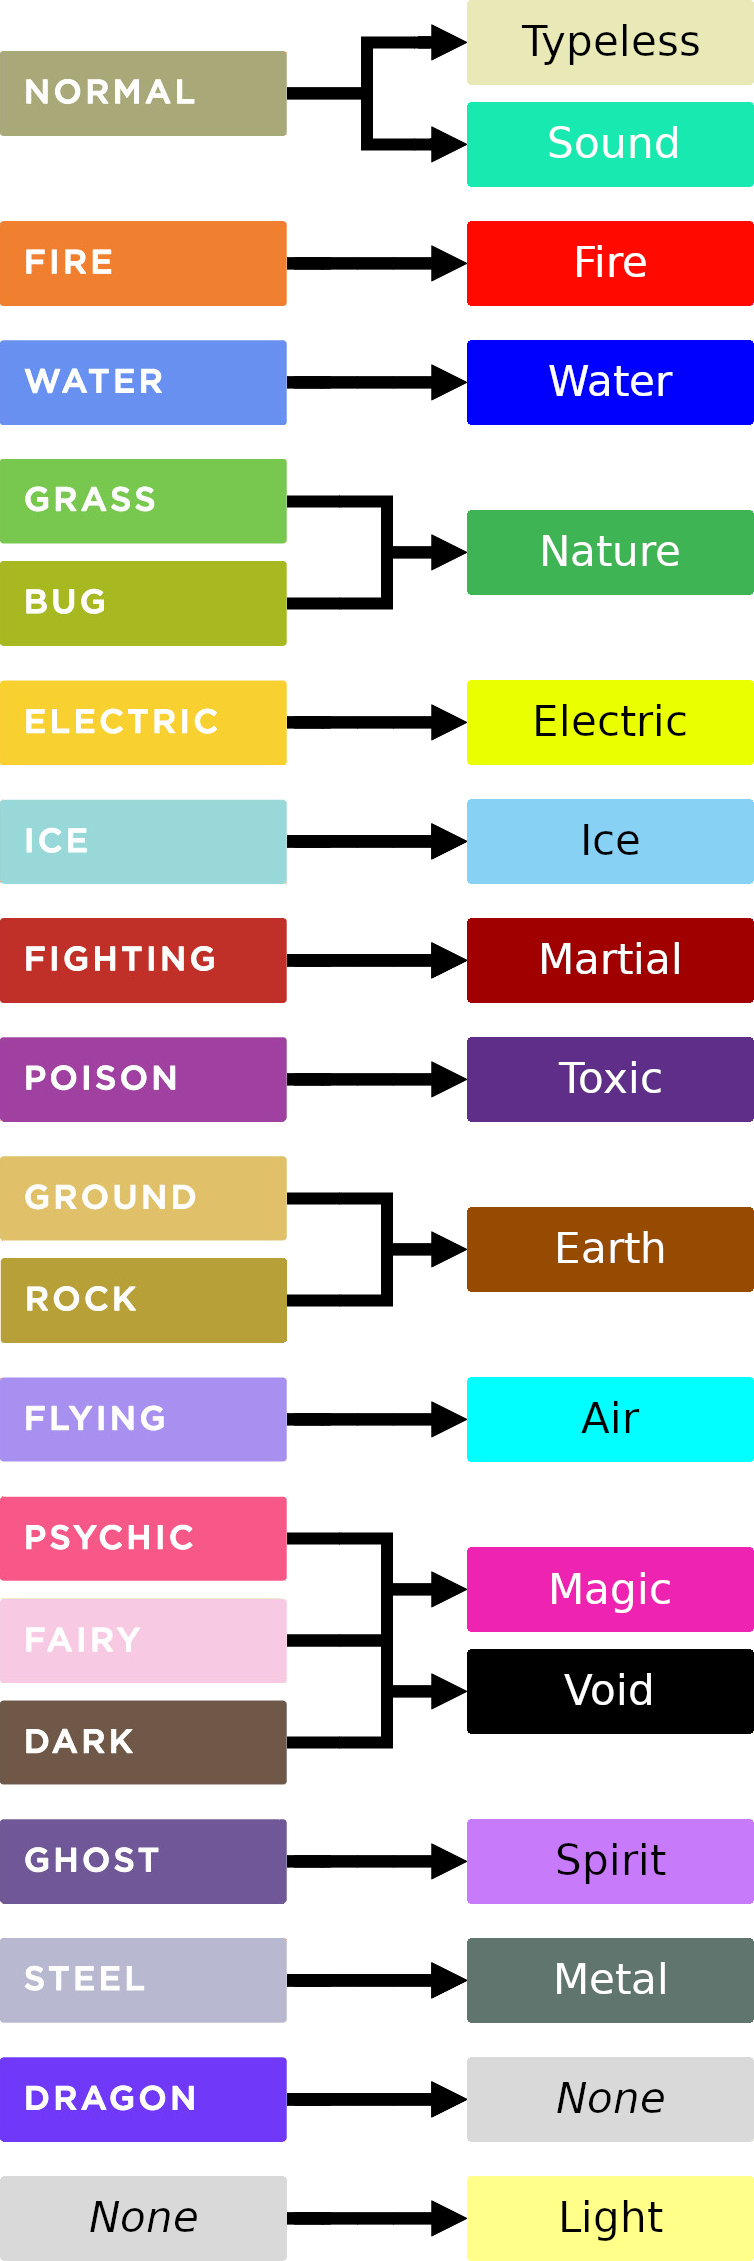
\includegraphics[scale=0.8]{map-from-pkmn}
	\caption{The 18 Pok\'{e}mon types (left) approximately mapped to the 16 Gene Hunter Types (right).}
\end{center}
\end{figure}

\sect{Fearsome Dual Types}


\begin{figure}
	\centering
	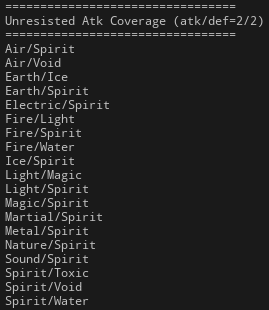
\includegraphics[scale=2]{unresisted-2v2}
	\caption{Dual Types that have unresisted coverage against dual Type defenders. Without Spirit, the list becomes [Air/Void], [Earth/Ice], [Fire/Light], [Fire/Water], and [Light/Magic].}
\end{figure}

\sect{Rock-Paper-Scissors}

\end{document}